\documentclass{beamer}
\mode<presentation>
\usepackage{amsmath,amssymb,mathtools}
\usepackage{textcomp}
\usepackage{gensymb}
\usepackage{adjustbox}
\usepackage{subcaption}
\usepackage{enumitem}
\usepackage{multicol}
\usepackage{listings}
\usepackage{url}
\usepackage{graphicx} % <-- needed for images
\def\UrlBreaks{\do\/\do-}

\usetheme{Boadilla}
\usecolortheme{lily}
\setbeamertemplate{footline}{
  \leavevmode%
  \hbox{%
  \begin{beamercolorbox}[wd=\paperwidth,ht=2ex,dp=1ex,right]{author in head/foot}%
    \insertframenumber{} / \inserttotalframenumber\hspace*{2ex}
  \end{beamercolorbox}}%
  \vskip0pt%
}
\setbeamertemplate{navigation symbols}{}

\lstset{
  frame=single,
  breaklines=true,
  columns=fullflexible,
  basicstyle=\ttfamily\tiny   % tiny font so code fits
}

\numberwithin{equation}{section}

% ---- your macros ----
\providecommand{\nCr}[2]{\,^{#1}C_{#2}}
\providecommand{\nPr}[2]{\,^{#1}P_{#2}}
\providecommand{\mbf}{\mathbf}
\providecommand{\pr}[1]{\ensuremath{\Pr\left(#1\right)}}
\providecommand{\qfunc}[1]{\ensuremath{Q\left(#1\right)}}
\providecommand{\sbrak}[1]{\ensuremath{{}\left[#1\right]}}
\providecommand{\lsbrak}[1]{\ensuremath{{}\left[#1\right.}}
\providecommand{\rsbrak}[1]{\ensuremath{\left.#1\right]}}
\providecommand{\brak}[1]{\ensuremath{\left(#1\right)}}
\providecommand{\lbrak}[1]{\ensuremath{\left(#1\right.}}
\providecommand{\rbrak}[1]{\ensuremath{\left.#1\right)}}
\providecommand{\cbrak}[1]{\ensuremath{\left\{#1\right\}}}
\providecommand{\lcbrak}[1]{\ensuremath{\left\{#1\right.}}
\providecommand{\rcbrak}[1]{\ensuremath{\left.#1\right\}}}
\theoremstyle{remark}
\newtheorem{rem}{Remark}
\newcommand{\sgn}{\mathop{\mathrm{sgn}}}
\providecommand{\abs}[1]{\left\vert#1\right\vert}
\providecommand{\res}[1]{\Res\displaylimits_{#1}}
\providecommand{\norm}[1]{\lVert#1\rVert}
\providecommand{\mtx}[1]{\mathbf{#1}}
\providecommand{\mean}[1]{E\left[ #1 \right]}
\providecommand{\fourier}{\overset{\mathcal{F}}{ \rightleftharpoons}}
\providecommand{\system}{\overset{\mathcal{H}}{ \longleftrightarrow}}
\providecommand{\dec}[2]{\ensuremath{\overset{#1}{\underset{#2}{\gtrless}}}}
\newcommand{\myvec}[1]{\ensuremath{\begin{pmatrix}#1\end{pmatrix}}}
\let\vec\mathbf

\title{Matgeo Presentation - Problem 1.2.10}
\author{ai25btech11004 - jaswanth}

\begin{document}


\frame{\titlepage}
\begin{frame}{Question}
Find the area of the triangle whose vertices are (-8,4),(-6,6) and (-3,9).
\end{frame}

\begin{frame}{Solution}

\begin{table}[h!]
	\centering
	\begin{table}[h!]
    \centering
    \begin{tabular}{|c|c|}
        \hline
        Point & Coordinates \\
        \hline
	    $A$ & $\myvec{1\\-1}$ \\
	    $B$ & $\myvec{-4\\2k}$ \\
	    $C$ & $\myvec{-k\\-5}$ \\
        \hline
    \end{tabular}
    \caption{Vertices of $\triangle ABC$ before substituting $k$}
    \label{tab:triangle_k}
\end{table}

	\caption{variables used}
	\label{}
\end{table}
\begin{align}
A-B = \myvec{-8 \\ 4} - \myvec{-6 \\ 6} 
= \myvec{-2 \\ -2},
\end{align}

\begin{align}
A-C = \myvec{-8 \\ 4} - \myvec{-3 \\ 9} 
= \myvec{-5 \\ -5}
\end{align}

\end{frame}
\begin{frame}{Solution}

Now, the area of the triangle is
\begin{align}
 \text{ar}(\triangle ABC) 
= \frac{1}{2} \left| (A-B) \times (A-C) \right|   
\end{align}

\begin{align}
 \text{ar}(\triangle ABC)=  \frac{1}{2} \left| \myvec{-2 \\ -2} \times  \myvec{-5 \\ -5} \right |
\end{align}



\begin{align}
\therefore \quad \text{ar}(\triangle ABC) = \frac{1}{2}(0) = 0
\end{align}


\noindent
Thus, the three points are collinear, and the triangle has area=0.
\end{frame}
\begin{frame}{Plot}
\begin{figure}[h]
    \centering
    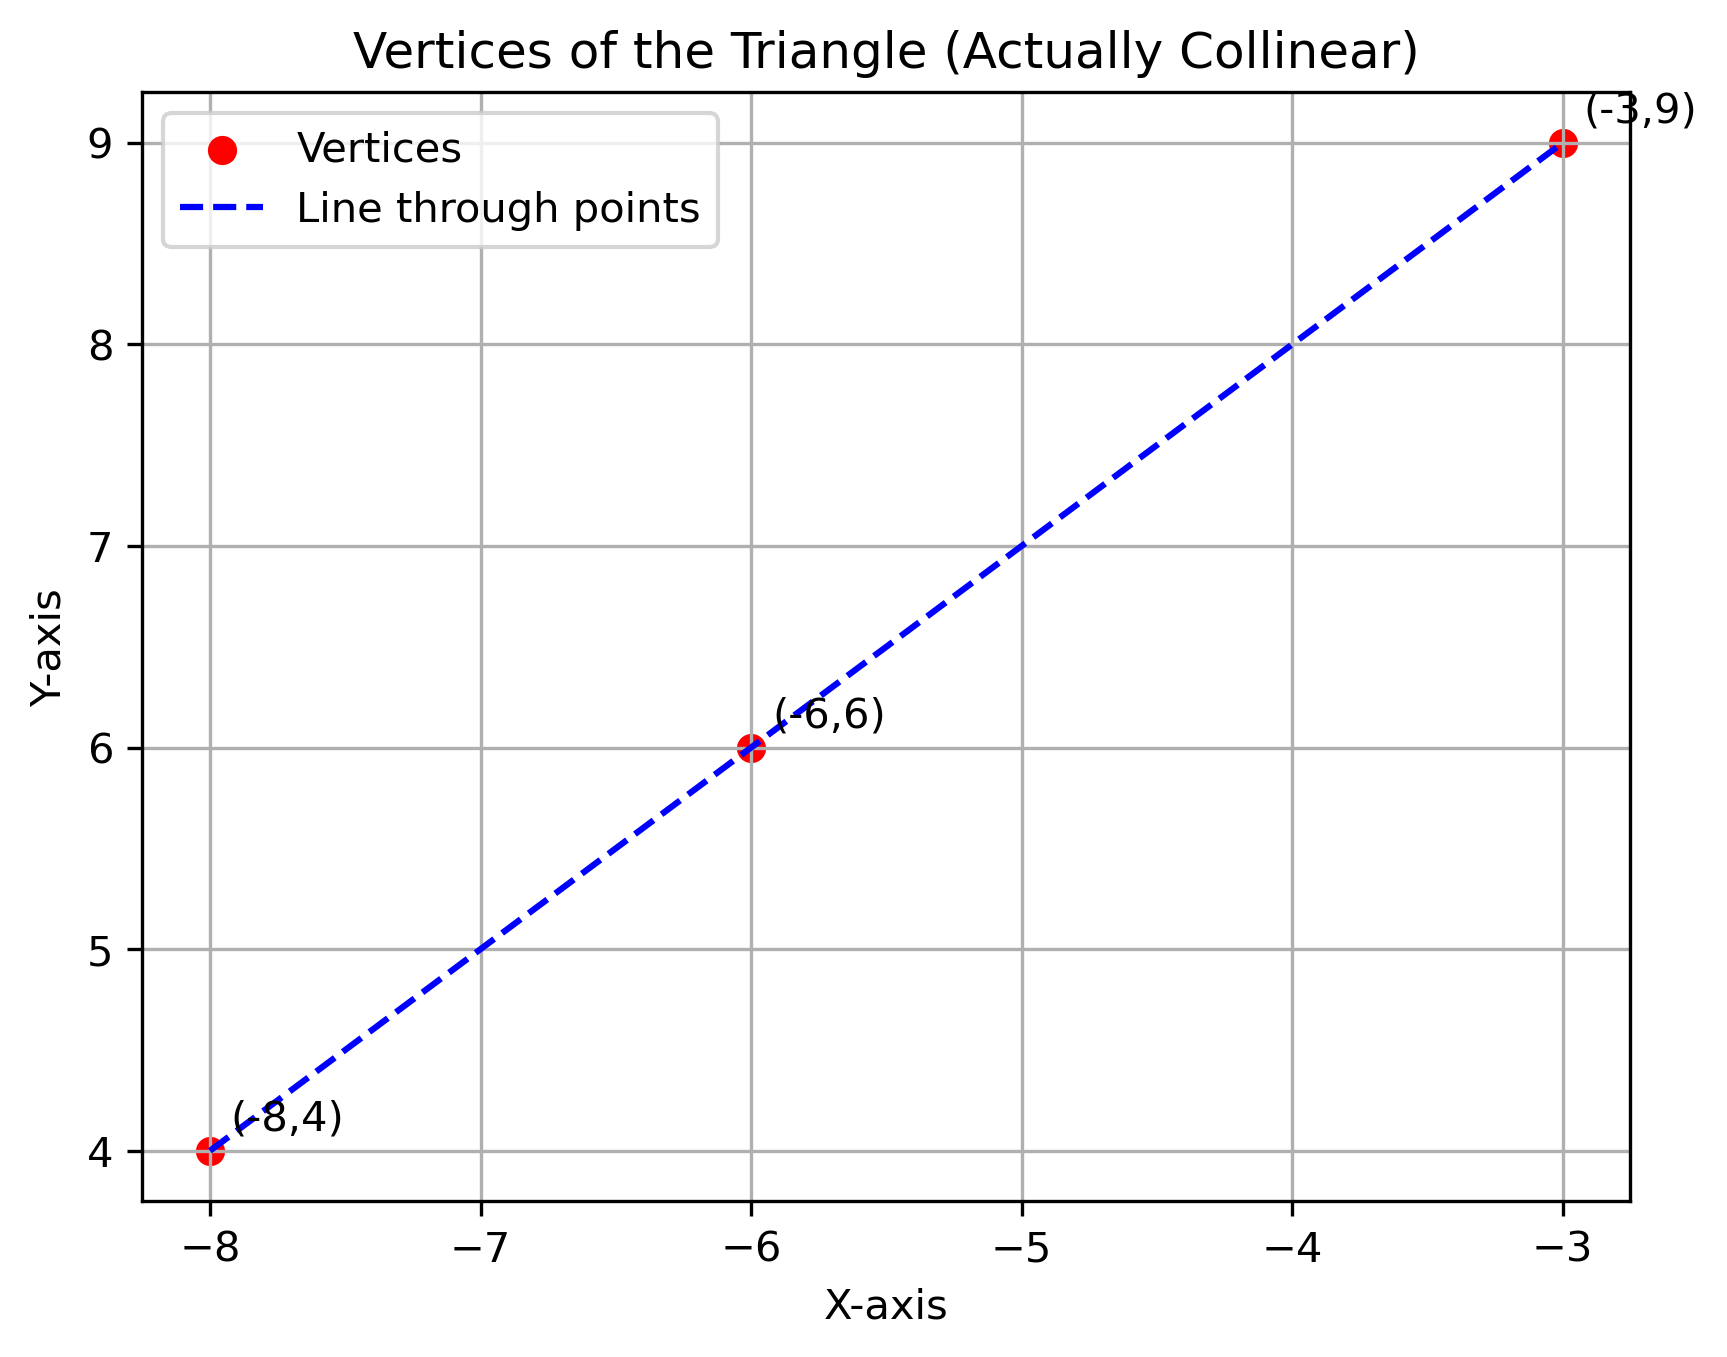
\includegraphics[width=0.5\linewidth]{figs/01.png}
    \caption{Caption}
    \label{fig:placeholder}
\end{figure}
\end{frame}
% --------- CODE APPENDIX ---------
\section*{Appendix: Code}

% C program
\begin{frame}[fragile]{C Code: code.c}
\begin{lstlisting}[language=C]
#include <stdio.h>
#include <stdlib.h>

int main() {
    // Coordinates of vertices
    int x1 = -8, y1 = 4;
    int x2 = -6, y2 = 6;
    int x3 = -3, y3 = 9;

    // Apply determinant formula for area
    float area = 0.5 * abs(x1*(y2 - y3) + x2*(y3 - y1) + x3*(y1 - y2));

    // Open file to write output
    FILE *fp = fopen("triangle.dat", "w");
    if (fp == NULL) {
        printf("Error opening file!\n");
        return 1;
    }

    fprintf(fp, "The area of the triangle is: %.2f\n", area);

    fclose(fp);

    printf("Output written to triangle.dat successfully.\n");

    return 0;
}

\end{lstlisting}
\end{frame}

% Python plotting
\begin{frame}[fragile]{Python: plot.py}
\begin{lstlisting}[language=Python]
import matplotlib.pyplot as plt

# Coordinates of the vertices
x = [-8, -6, -3]
y = [4, 6, 9]

# Plot points
plt.scatter(x, y, color='red', label='Vertices')

# Connect the points (straight line since collinear)
plt.plot(x, y, color='blue', linestyle='--', label='Line through points')

# Annotate the points
for i, txt in enumerate([f"({x[i]},{y[i]})" for i in range(len(x))]):
    plt.annotate(txt, (x[i], y[i]), textcoords="offset points", xytext=(5,5))

# Labels and title
plt.xlabel("X-axis")
plt.ylabel("Y-axis")
plt.title("Vertices of the Triangle (Actually Collinear)")
plt.legend()
plt.grid(True)

# Save the figure
plt.savefig("triangle.png", dpi=300, bbox_inches="tight")

# Close the figure to free memory
plt.close()

print("Graph saved as triangle.png")



\end{lstlisting}
\end{frame}
\end{document}



